\chapter{Architecture Exploration}\label{models}
This chapter presents the proposed neural network architectures. It starts with a baseline TNN network, which then undergoes a series of hardware-aware adaptions specific to jet tagging. During this process two separate architectures are developed, which differ by the input type and design goal. The first one, referred to as the \textit{ultra-low latency} one, targets the HLF jet representation and aims to achieve the lowest possible latency at the cost of accuracy and AUC values. The second one, called \textit{accuracy-focused}, is based on the constituent list jet representation and trade-offs latency for quality of classification while still remaining within L1T timing constraints.


\section{Baseline Software Architecture}
The starting point of this analysis is derived from transformer architecture used in the original paper \cite{44-vaswani2017attention} and recent proof-of-concept used for jet tagging \cite{3-yuan2021constituentnet:}. The overview of the network components can be seen in figure \ref{fig:constituent-net}.

\begin{figure}[hpt!]
  \centering
  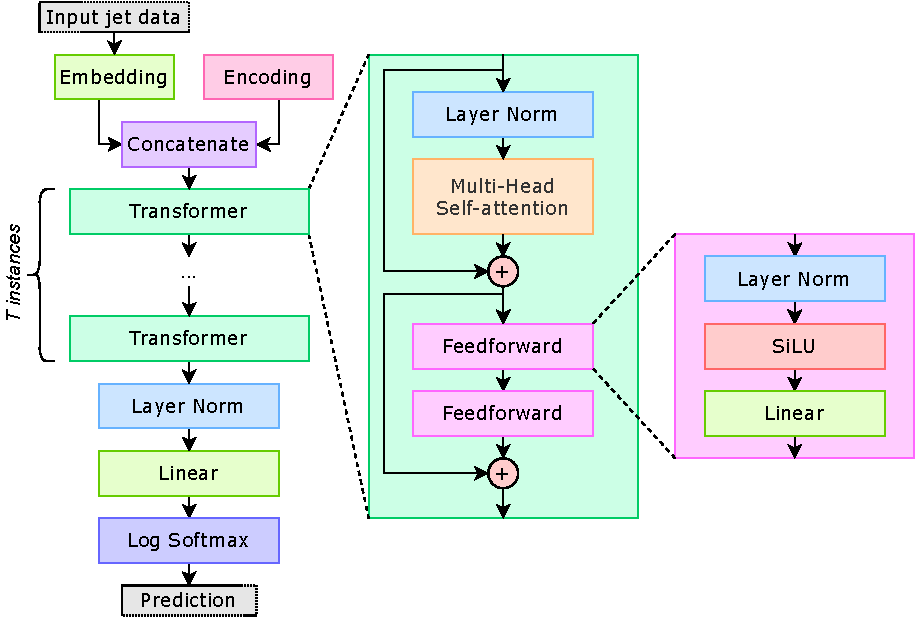
\includegraphics[trim={0cm 0cm 0cm 0cm}, width=0.6\textwidth, center]{models/constituent_net.pdf}
  \caption{Diagram with an overview of the baseline architecture.}
  \label{fig:constituent-net}
\end{figure}

The straight-forward path between model's input and output highlights the sequential nature of transformer which stands in opposition to recurrency present in GRU and LSTM models. While this allows for the aforementioned parallelizability and pipelining on FPGAs, it also poses a challenge of increased hardware footprint and synthesis complexity when compared to recurrent models, where the key components can get reused to meet the resource constraints. To better understand the transformer's complexity, the next subsections derive the equations linking the internal components and explain the involved terminology.


\subsection{Input embedding and Residual Connections}
Although the model lacks any recurrency, the transformer includes two residual connections which have been widely adopted since their successful application in ResNet neural networks \cite{75-kaiming2016deep}. They offer improvements to training time and resulting accuracy \cite{74-szegedy2016inception-v4}, however, they require standardized data dimensionality to ensure the summation can be logically executed. In this project, this is obtained thanks to input embedding, which transforms the input \(\bm{\hat{x^i}} \in \mathbb{R}^{L \times 16} \) into a shape \(\mathbb{R}^{L \times d}\) that is used through the design, as seen in equation \ref{eq:embedding}.

\begin{equation}\label{eq:embedding}
  \bm{\hat{x^i}_{\text{emb}}} = \text{embedding} ( \bm{\hat{x^i}} ) = w_{\text{embed}}\; \bm{\hat{x^i}} + b_{\text{embed}} \in \mathbb{R}^{L \times d}
\end{equation}

This dimensionality change can be conveniently performed using a linear layer, and it has to be remembered that each such layer increased the model learning capacity thanks to the learnable weights and bias. The network's inner dimension \(d\) is treated as a hyperparameter as it influences the model's accuracy and performance, but it has to be noted that the other dimension prevalent in the network comes from the input's number of jet constituents \(L\) (which is set to 1 in case of the HLS representation), meaning that the model is also susceptible to a parameter which cannot be easily tuned.

\subsection{Input Encoding}
Along the embedding, an input encoding is concatenated and fed to the transformer layer. In natural language processing, the encoding is meant to allow the model to benefit from the sequential information of the words in a sentence. It can be obtained from a sinusoidal function using the position index or simply treated as another learnable parameter. The sequential relations are not present in the jet data, because all the jets originate from the same proton-proton collision, hence, the latter approach is used in this project. It is worth mentioning, that from empirical analysis, the learnable encodings have a significant impact on the final results as they represent a trained, hidden state concatenated to all inputs during evaluation, as shown in equation \ref{eq:encoding}. Its impact is especially prevalent for the HLF data (where \(L = 1\)), where the hidden state matched input's dimension and effectively doubles it after concatenation.

\begin{equation}\label{eq:encoding}
  \text{encoding} ( \bm{\hat{x^i}_{\text{emb}}} ) = w_{\text{encoding}} \in \mathbb{R}^{1 \times d} \implies \text{concat} (\bm{\hat{x^i}_{\text{emb}}},\; w_{\text{encoding}}) \in \mathbb{R}^{(L+1) \times d}
\end{equation}

Choosing a learned hidden state is also more efficient for inference in hardware, as the increased training cost associated with back-propagation of this parameter yields a constant set of values that are known during compile-time of the FPGA and can be implemented using a LUT.

\subsection{Normalization}
 make transformer layers ... instead of 1 or 3 in baseline diagram?

\section{Ultra-Low Latency Architecture}

\subsection{Simplification and Tuning}

\subsection{Hardware Mapping}


\section{Accuracy-Focused Architecture}

\subsection{Hardware Mapping}


\section{Parameter Extraction for Custom Hardware}
\indo{tool for extracting weight and biases}

In order to generate files with weights and biases that are required for initializing the memory on an FPGA, a tool was developed that takes a PyTorch pre-trained model, extracts all the information, and splits them accordingly with the required format. What is more, layers responsible for normalization can be chosen to have their mean and variance calculation embedded into weights and biases to significantly reduce the processing required on an FPGA by omitting the division and square root operations. The mathematical derivation of this approach starts with the batch norm formula:
\[ y = \frac{x - E[x]}{\sqrt{Var[x] + \epsilon}} * \gamma + \beta \]
The expected value and variance are treated as learnable parameter of a dataset and are extracted after the training has been completed. Hence, the calculation becomes:
\[ y = x * \frac{\gamma}{\sqrt{Var + \epsilon}} + \beta - \frac{\gamma * E}{\sqrt{Var + \epsilon}} = x * W + b\]
The newly calculated values for \(W\) and \(b\) represent the updated weights and biases of the normalization layer, that can be then implemented in hardware in a much simpler way. Independently of the implementation in this work, a similar idea has been proposed and successfully used as an optimization in the past \cite{46-fan2018real-time}.

\indo{tool for embedding norm stats for layer norm as running stats not collected}

\indo{stability issues solved by more normalization (coming from wide range of inputs of 30x16)}
